\chapter{Cold free fermion neutron stars}

\TODO{better title}

\TODO{inspiration, references}

\TODO{intro}

In \cref{chap:tft}, we found $Z = Z(T, \mu, V)$ for two sample systems, and in particular a gas of free Dirac fermions.
From $Z$, we can derive the pressure $P = P(T, \mu)$ and energy density $\epsilon = \thermalavg{E}/V = \epsilon(T, \mu)$ using \cref{eq:tft:average_number,eq:tft:average_energy,eq:tft:average_pressure}, where the volume $V$ has been eliminated by division, because $P$ and $\epsilon$ are intensive quantities.
At some fixed temperature $T$, we can therefore eliminate $\mu$ to express $\epsilon$ in terms of $P$.
This gives us an equation of state $\epsilon = \epsilon(P)$ with which we can solve the Tolman-Oppenheimer-Volkoff system \eqref{eq:tov:tovsys}.

In this chapter, we will use partition function \eqref{eq:tft:dirac_partition_function} for free Dirac fermions and do exactly this to model a neutron star with a cold ideal Fermi gas of neutrons.
\TODO{bad wording: use something like ``equation of state for free/ideal cold fermi gas?}

\section{Equation of state}

For easy reference, the logarithm of the free Dirac fermion partition function \eqref{eq:tft:dirac_partition_function} is
\begin{equation}
	\log Z = 2 V \int \frac{\dif^3 p}{(2 \pi \hbar)^3} \bigg\{ \beta E(\vec{p}) + \log \left[ e^{-\beta (E(\vec{p}) - \mu)}+1 \right] + \log \left[ e^{-\beta (E(\vec{p}) + \mu)} + 1\right] \bigg\}.
\end{equation}
First, the particle number density $n = \thermalavg{N}/V$ follows from the derivative \eqref{eq:tft:average_number} and is
\begin{equation}
	n = 
	\frac{1}{\beta} \pdv{\log Z}{\mu} =
	2 \int \frac{\dif^3 p}{(2 \pi \hbar)^3} \Big\{ n\big[ E(\vec{p})-\mu \big] - n\big[ E(\vec{p})+\mu \big] \Big\} ,
\label{eq:nstars:density}
\end{equation}
where we defined the \textbf{Fermi-Dirac distribution}
\begin{equation}
	n(E) = \frac{1}{e^{-\beta E} + 1}.
\label{eq:nstars:fermi_dirac_distribution}
\end{equation}
Do not confuse the particle density $n$ on the left with the Fermi-Dirac distributions $n[E(\vec{p}) \mp \mu]$ on the right!
We will soon perform the integral over $\vec{p}$ and get rid of $n[E(\vec{p}) \mp \mu]$, anyway.
From the density \eqref{eq:nstars:density}, we see that $n = n(\mu, T)$ is a function of the chemical potential $\mu$ and temperature $T$, so that at some fixed temperature, the value of $\mu$ determines the particle density $n$.

Second, we calculate the energy density $\epsilon = \thermalavg{E} / V$ from \cref{eq:tft:average_energy}.
It comes out as \TODO{different wording}
\begin{equation}
	\epsilon = 
	\mu n - \frac{1}{V} \pdv{\log Z}{\beta} =
	2 \int \frac{\dif^3 p}{(2 \pi \hbar)^3} \Big\{ -E(\vec{p}) + E(\vec{p}) \, n\big[ E(\vec{p})-\mu \big] + E(\vec{p}) \, n\big[ E(\vec{p})+\mu \big] \Big\}.
\label{eq:nstars:energy_density}
\end{equation}

Third, we find that the pressure \eqref{eq:tft:average_pressure} is
\begin{equation}
	P =
	\frac{\log Z}{\beta V} = 
	2 \int \frac{\dif^3 p}{(2 \pi \hbar)^3} \bigg\{ E(\vec{p}) + \log \left[ e^{-\beta(E(\vec{p})-\mu)} + 1 \right] + \log \left[ e^{-\beta(E(\vec{p})+\mu)} + 1 \right] \bigg\}.
\label{eq:nstars:pressure}
\end{equation}

The first term of the energy density \eqref{eq:nstars:energy_density} and the pressure \eqref{eq:nstars:pressure} is infinite, as the integrand never decays \TODO{decay usually associated with radiation}.
This can be interpreted as an infinite shift of the vacuum energy.
In contrast, the two last terms are finite as the integrand is suppressed \TODO{?} for large $\abs{\vec{p}}$ by the Fermi-Dirac distribution.
It makes no sense to include a term that integrates over every possible value of the momentum $\vec{p}$ for physical particles whose momentum cannot exceed a certain value due to energy conservation.
Here, we will make the assumption that we can simply drop the infinite term.
We will return later to investigate this term by regularization and renormalization. \TODO{does this make sense?} \TODO{improve convergence/divergence arguments, look at measure $p^2$, etc.}

From the particle density \eqref{eq:nstars:density} at constant temperature $T$, we see that the sign of $n$ is determined by the sign of $\mu$.
The total density $n$ is expressed as a balance between \emph{particles} with energy $E(\vec{p}) > 0$ living relative to the chemical potential $\mu$ and \emph{antiparticles} with energy $E(\vec{p}) < 0$ living relative to the chemical potential $-\mu$.
Thus, the chemical potential $\mu$ determines the balance between particles and antiparticles in the system.
Similarly, the two last terms in the energy density \eqref{eq:nstars:energy_density} and pressure \eqref{eq:nstars:pressure} can be interpreted as contributions from particles and antiparticles.
We choose a large, positive value of $\mu > 0$, so that the particles dominate the system, while antiparticles are hardly present.
With this choice, $n \left[ E(\vec{p}) - \mu \right] \gg n \left[ E(\vec{p}) + \mu \right]$, and we drop the last term from the particle density \eqref{eq:nstars:density}, energy density \eqref{eq:nstars:energy_density} and pressure \eqref{eq:nstars:pressure}.

Dropping terms as described in the last paragraphs, we are left with the%
\begin{subequations}%
\begin{align}%
	& \text{particle density} & n        &=  2 \int \frac{\dif^3 p}{(2 \pi \hbar)^3} \, n \left[ E(\vec{p})-\mu \right] ,                    \label{eq:nstars:dropped_infinities_density} \\
	& \text{energy density}   & \epsilon &=  2 \int \frac{\dif^3 p}{(2 \pi \hbar)^3} \, E(\vec{p}) \, n \left[ E(\vec{p})-\mu \right] ,      \label{eq:nstars:dropped_infinities_energy_density} \\
	& \text{pressure}         & P        &= -2 \int \frac{\dif^3 p}{(2 \pi \hbar)^3} \, \log \left[ e^{-\beta(E(\vec{p})-\mu)} + 1 \right] . \label{eq:nstars:dropped_infinities_pressure}
\end{align}%
\label{eq:nstars:dropped_infinities}%
\end{subequations}%
The integrals become nasty after plugging in the relativistic dispersion relation \eqref{eq:tft:dispersion} and the Fermi-Dirac distribution \eqref{eq:nstars:fermi_dirac_distribution}, and it is overly optimistic to expect that all of them can be evaluated analytically.
We will make one final approximation that will make all the integrals surmountable.

\TODO{what about $\beta \mu \gg 1$? assume/take this into account.}
By human standards, it is very hot inside a neutron star.
In fact, studies estimate typical core temperatures around $T_0 \approx \SI{1e6}{\kelvin}$. \TODO{reference}
However, neutrons have mass $m \approx \SI{1.67e-27}{\kilogram}$, so everywhere inside a neutron star we have $\beta E(\vec{p}) = \sqrt{\vec{p}^2 c^2 + m^2 c^4} / k_B T > m c^2 / k_B T_0 \approx 10^7 \gg 1$.
Although the temperature is very large compared to everyday temperatures, the thermal energy $k_B T$ is in fact very low relative to the energy $E(\vec{p})$ of the nuclei.
It is therefore an excellent approximation to take the \textbf{zero-temperature limit}
\begin{equation}
	\beta E(\vec{p}) \gg 1 .
\end{equation}

\begin{figure}
	\centering
	\begin{tikzpicture}
		\begin{groupplot}[group style={group size=2 by 1, horizontal sep=5pt}, height=6cm, width=7cm, /tikz/declare function={
			n(\b,\E) = 1/(exp(\b*\E)+1);
		}]
			\nextgroupplot[xlabel=$E$, ylabel=$1/(e^{\beta E}+1)$, 
				colorbar horizontal, colorbar sampled, colorbar style={xlabel=$\beta$, samples=7, xtick={-0.5, 0.5, 1.5, 2.5, 3.5, 4.5}, xticklabels={$1/2$, $1$, $2$, $4$, $8$, $16$, $32$}, grid=none, xticklabel pos=upper, tickwidth=0, at={(0.0,1.03)}, anchor=south west},
				every colorbar/.append style={width=2*\pgfkeysvalueof{/pgfplots/parent axis width}+\pgfkeysvalueof{/pgfplots/group/horizontal sep}},
				xtick distance=10, ytick distance=0.5, grid=none, minor tick num=1,
			]
			\pgfplotsinvokeforeach{0.5, 1, 2, 4, 8, 16, 32}{
				\addplot[domain=-10:+10, samples=200, mesh, point meta={log2(#1)}] {n(#1, x)};
			}

			\nextgroupplot[xlabel=$E$, ylabel=$\log (e^{-\beta E}+1)/\beta$, xtick distance=10, yticklabel pos=right, ytick distance=5, minor tick num=1, grid=none]
			\pgfplotsinvokeforeach{0.5, 1, 2, 4, 8, 16, 32}{
				\addplot[domain=-10:+10, samples=200, mesh, point meta={log2(#1)}] {ln(exp(-#1*x)+1)/#1};
			}
		\end{groupplot}
	\end{tikzpicture}
\caption{\label{fig:nstars:distribution_convergence}%
	In the zero-temperature limit $\beta E \gg 1$, the Fermi-Dirac distribution $1/(e^{\beta E}+1) \rightarrow \theta(-E)$, while $\log (e^{-\beta E} + 1) \rightarrow -\beta E \, \theta(-E)$, where $\theta(E)$ is the step function.
}
\end{figure}

In the zero-temperature limit, the Fermi-Dirac distribution can be replaced by
\begin{equation}
	n(E)       =                 \begin{cases} 1 / (e^{+\beta \abs{E}}+1) & (E>0) \\ 1 / (e^{-\beta \abs{E}}+1) & (E<0) \end{cases}
	     \quad \rightarrow \quad \begin{cases} 0 & (E>0) \\ 1 & (E<0) \end{cases}
	     \quad =                 \theta(-E) ,
\end{equation}
while the logarithm in the pressure behaves as
\begin{equation}
	\log (e^{-\beta E}+1)       =                 \begin{cases} \log (e^{-\beta \abs{E}}+1) & (E>0) \\ \log (e^{+\beta \abs{E}}+1) & (E<0) \end{cases}
	                      \quad \rightarrow \quad \begin{cases} \log 1 & (E>0) \\ \log e^{-\beta E} & (E<0) \end{cases}
	                      \quad =                 -\beta E \, \theta(-E) .
\end{equation}
This is confirmed by the plots in \cref{fig:nstars:distribution_convergence} for increasing values of $\beta$.
Thus, the zero-temperature limit effectively limits the integrals \eqref{eq:nstars:dropped_infinities} to those momenta $\vec{p}$ with $E(\vec{p}) < \mu$.
We therefore call
\begin{equation}
	\mu = E_F = E(p_F) = \sqrt{p_F^2 c^2 + m^2 c^4}
\end{equation}
the Fermi energy and the corresponding momentum $p_F$ the Fermi momentum, representing the occupied state in momentum-space with largest energy and momentum.

Now the particle density \eqref{eq:nstars:dropped_infinities_density} simply becomes
\begin{equation}
	n = 
	2 \int_0^\infty \frac{\dif p \, 4 \pi p^2}{(2 \pi \hbar)^3} \theta \left[ \mu - E(p) \right] =
	2 \int_0^{p_F} \frac{\dif p \, 4 \pi p^2}{(2 \pi \hbar)^3} = \frac{p_F^3}{3 \pi^2 \hbar^3} .
\label{eq:nstars:density_zeroT}
\end{equation}
Using integral \TODO{ref} and defining the dimensionless momentum $x = p / mc$, the energy density \eqref{eq:nstars:dropped_infinities_energy_density} is
\begin{equation}
\begin{split}
	\epsilon &=  2 \int_0^\infty \frac{\dif p \, 4 \pi p^2}{(2 \pi \hbar)^3} \, E(p) \, \theta \left[ \mu - E(p) \right] \\
	         &=  2 \int_0^{p_F} \frac{\dif p \, 4 \pi p^2}{(2 \pi \hbar)^3} \, \sqrt{p^2 c^2 + m^2 c^4} \\
	         &= \frac{m^4 c^5}{\pi^2 \hbar^3} \int_0^{x_F} \dif x \, x^2 \sqrt{1 + x^2} \\
	         &= \frac{m^4 c^5}{8 \pi^2 \hbar^3} \left[ \left( 2 x_F^3 + x_F \right) \sqrt{1 + x_F^2} - \asinh x_F \right] . \\
\end{split}
\label{eq:nstars:energy_density_zeroT}
\end{equation}
Finally, using the same integral, the pressure \eqref{eq:nstars:dropped_infinities_pressure} is
\begin{equation}
\begin{split}
	P &= \frac{2}{\beta} \int_0^\infty \frac{\dif p \, 4 \pi p^2}{(2 \pi \hbar)^3} \, \beta \left[ \mu - E(p) \right] \, \theta \left[ \mu - E(p) \right] \\
	  &= 2 \int_0^{p_F} \frac{\dif p \, 4 \pi p^2}{(2 \pi \hbar)^3} \, \left[ \sqrt{p_F^2 c^2 + m^2 c^4} - \sqrt{p^2 c^2 + m^2 c^4} \right] \\
	  &= \frac{m^4 c^5}{\pi^2 \hbar^3} \int_0^{x_F} \dif x \, x^2 \left[ \sqrt{x_F^2+1} - \sqrt{x^2+1} \right] \\
	  &= \frac{m^4 c^5}{24 \pi^2 \hbar^3} \left[ \left( 2 x_F^3 - 3 x_F \right) \sqrt{x_F^2 + 1} + 3 \asinh x_F \right] . \\
\end{split}
\label{eq:nstars:pressure_zeroT}
\end{equation}

The equation of state $\epsilon = \epsilon(P)$ follows by eliminating $x_F$ from the energy density \eqref{eq:nstars:energy_density_zeroT} and pressure \eqref{eq:nstars:pressure_zeroT}.
Due to their complicated dependence on $x_F$, we will do so in three cases of increasing difficulty.

\TODO{first present three cases, \emph{then} do calculations, to not overload the reader}

\subsection{Ultra-relativistic limit}
\label{sec:nstars:ur_limit}

First, consider the ultra-relativistic limit
\begin{equation}
	x_F \gg 1 , 
\label{eq:nstars:ur_limit}
\end{equation}
where the Fermi energy $E_F = \sqrt{p_F^2 c^2 + m^2 c^4} \taylor p_F c$ is dominated by the contribution from the Fermi momentum.
Since $\asinh x_F = \log \left[ x_F + \sqrt{x_F^2 + 1} \right] \taylor \log 2 x_F$ diverges logarithmically, we see that both the energy density \eqref{eq:nstars:energy_density_zeroT} and pressure \eqref{eq:nstars:pressure_zeroT} are dominated by their first term with $2 x_F^3 \sqrt{x_F^2 + 1} \taylor 2 x_F^4$.
In the ultra-relativistic limit, then,
\begin{equation}
	\epsilon \taylor \frac{m^4 c^5 x_F^4}{4 \pi^2 \hbar^3}
	\qquad \text{and} \qquad
	P        \taylor \frac{m^4 c^5 x_F^4}{12 \pi^2 \hbar^3},
\end{equation}
and $x_F$ is easily eliminated, yielding the very simple equation of state
\begin{equation}
	\epsilon = 3 P .
\label{eq:nstars:ur_eos}
\end{equation}

In this particular case, the TOV system \eqref{eq:tov:tovsys} can be solved analytically with the polynomial trial solution
\begin{equation}
	P(r) = A r^n .
\label{eq:nstars:ur_ansatz}
\end{equation}
Then the mass equation \eqref{eq:tov:tovsys_mass} is
\begin{equation}
	\odv{m}{r} = \frac{12 \pi A}{c^2} r^{n+2},
	\qquad \text{so} \qquad
	m(r) = \frac{12 \pi A}{(n+3) c^2} r^{n+3}
	\quad (n \neq -3).
\label{eq:nstars:ur_mass}
\end{equation}
With the equation of state \eqref{eq:nstars:ur_eos}, mass \eqref{eq:nstars:ur_mass} and trial solution \eqref{eq:nstars:ur_ansatz}, the TOV equation \eqref{eq:tov:tovsys_pressure} reads
\begin{equation}
	n A r^{n-1} =
	-\frac{48 \pi G A^2 r^{2n+1}}{(n+3) c^4} \left[ 2 + \frac{n}{3} \right] \left[ 1 - \frac{24 \pi G A r^{n+2}}{(n+3) c^4} \right]^{-1} .
\end{equation}
We can attain equality for all $r$ if we choose $n = -2$.
Then the rightmost factor no longer depends on $r$, and both sides have the same $r^{-3}$-dependence
\begin{equation}
	- 2 A r^{-3} = - \frac{64 \pi G A^2 r^{-3}}{c^4} \left[ 1 - \frac{24 \pi G A}{c^4} \right]^{-1} .
\end{equation}
Equality is established if we match the prefactors by choosing $A = c^4 / 56 \pi G$.
Then the solutions for the pressure and mass are
\begin{equation}
	P(r) = \frac{c^4}{56 \pi G} \frac{1}{r^2}
	\qquad \text{and} \qquad
	m(r) = \frac{3 c^2}{14 G} r .
\end{equation}
This is a highly unphysical result.
The pressure diverges at the center, so nothing could ever hold such a star together.
In addition, $p(r) > 0$ for all $r$, so the star has no surface and hence infinite mass $M = m(\infty) = \infty$.

\TODO{make plot of $P(r)$ and $m(r)$ for a star.}

\subsection{Non-relativistic limit}
\label{sec:nstars:nr_limit}

Next, let us consider the more difficult non-relativistic limit
\begin{equation}
	x_F \ll 1,
\label{eq:nstars:nr_limit}
\end{equation}
where the Fermi energy $E_F = \sqrt{p_F^2 c^2 + m^2 c^4} \taylor m c^2$ is dominated by the rest energy of the fermions.
Taylor expanding the energy density \eqref{eq:nstars:energy_density_zeroT} and presure \eqref{eq:nstars:pressure_zeroT} around $x_F = 0$ to lowest order, we find
\begin{equation}
	%\epsilon &\taylor \frac{m c^2 p_F^3}{3 \pi^2 \hbar^3} + \frac{p_F^5}{10 \pi^2 \hbar^3 m} = n m c^2 + \frac{p_F^5}{10 \pi^2 \hbar^3 m} \\
	%P        &\taylor \frac{p_F^5}{15 \pi^2 \hbar^3 m}
	\epsilon \taylor \frac{m c^2 p_F^3}{3 \pi^2 \hbar^3}
	\qquad \text{and} \qquad
	P        \taylor \frac{p_F^5}{15 \pi^2 \hbar^3 m} .
\end{equation}
Note that with the density \eqref{eq:nstars:density}, the energy density can be written $\epsilon = n m c^2$, so it is only due to the rest mass of the particles, as if all fermions have broken free from the Pauli exclusion principle and possess the same rest energy $m c^2$.
This is only a mathematical feature of the non-relativistic limit -- the fermions still occupy different states with different momentum, but the momenta are so small that the differences are negligible compared to the rest energy $mc^2$.
Again, it is straightforward to eliminate $x_F$ to find the equation of state, only this time there is some extra bookkeeping with all the exponents.
Carefully gathering all the prefactors under the same roof, we find
\begin{equation}
	%\epsilon = \frac{mc^2}{3\pi^2\hbar^3} \left( 15 \pi^2 \hbar^3 m P \right)^{3/5}
	\epsilon = \left( \frac{5^3 m^8 c^{10}}{3^2 \pi^4 \hbar^6} \right)^{\frac15}  P^{\frac35} .
\end{equation}
With this power dependence, it is not easy, if even possible, to solve the TOV equation analytically.
The trial solution \eqref{eq:nstars:ur_ansatz} we employed in \cref{sec:nstars:ur_limit} fails miserably, as we do not get the same fortunate cancellations of $r$.
We therefore resort to the numerical solution method described in \cref{sec:nstars:numtov}, parametrizing different stars by their center pressure $P_0$ and integrating the TOV equation until the pressure $p(R)$ vanishes, using the corresponding radius $R$ to establish the mass $M = m(R)$ of the star.
The results are shown in \cref{fig:nstars:massradius}.

\iffalse
Dimensionless equation of state
\begin{equation}
	\diml{\epsilon} = \left[ \frac{4^2 5^3}{3^4 \pi^2} \frac{m^8 c^6 r_0^6}{m_0^2 \hbar^6} \diml{P}^3 \right]^{\frac{1}{5}}
\end{equation}
\fi

\subsection{General Fermi momenta}
\label{sec:nstars:gr_limit}

How can we find the energy density
\begin{equation}
	\epsilon = \frac{m^4 c^5}{8 \pi^2 \hbar^3} \left[ \left( 2 x_F^3 + x_F \right) \sqrt{1 + x_F^2} - \asinh x_F \right]
\label{eq:nstars:gr_limit_energy_density}
\end{equation}
that corresponds to a given pressure
\begin{equation}
	P = \frac{m^4 c^5}{24 \pi^2 \hbar^3} \left[ \left( 2 x_F^3 - 3 x_F \right) \sqrt{x_F^2 + 1} + 3 \asinh x_F \right] 
\label{eq:nstars:gr_limit_pressure}
\end{equation}
for general $x_F$?
Since we are already solving the TOV equation on a computer, we can do so by numerical root finding.
At every step $r$ in the numerical integration algorithm, we know the current pressure $P = P(r)$.
Using a numerical root finding algorithm, we can find the root $x_F$ of the function
\begin{equation}
	f(x_F) = P(x_F) - P = 0,
\end{equation}
where $P(x_F)$ is the pressure \eqref{eq:nstars:gr_limit_pressure} as a function of $x_F = p_F / m c$.
Having found the root, we can simply calculate the corresponding energy density $\epsilon(x_F)$ from \cref{eq:nstars:gr_limit_energy_density}.
This whole procedure can be elegantly encapsulated into a function that implements an implicit equation of state $\epsilon = \epsilon(P)$, which in turn is straightforward to plug into our solver described in \cref{sec:nstars:numtov}.
The results are shown in \cref{fig:nstars:massradius}.

\iffalse
\begin{equation}
	\diml{P}(x_F) = \frac{m^4 c^3 r_0^3}{18 \pi m_0 \hbar^3} \left[ (2 x_F^3 - 3 x_F) \sqrt{x_F^2 + 1} + 3 \asinh x_F \right]
\end{equation}

At every integration step, we have a value of the pressure $P$.
Then find the root $x_F$ of
\begin{equation}
	P(x_F) - P = 0
\end{equation}
and then calculate
\begin{equation}
	\diml{ϵ} = \diml{ϵ}(x_F) = \diml{P}(x_F) = \frac{m^4 c^3 r_0^3}{6 \pi m_0 \hbar^3} \left[ (2 x_F^3 + x_F) \sqrt{x_F^2 + 1} - \asinh x_F \right]
\end{equation}
\fi

\tablemaximum{../code/data/nr.dat}{M}{\maxMnr}{R}{\maxRnr}
\tablemaximum{../code/data/gr.dat}{M}{\maxMgr}{R}{\maxRgr}

\begin{figure}
\centering
\begin{tikzpicture}
\begin{axis}[
	width=15cm, height=10cm,
	xlabel=$R / \si{\kilo\meter}$, ylabel=$M / \solarmass$, title={Mass-radius relation for cold free Fermi gas neutron star}, title style={yshift=1.8cm},
	grid=major,
	colorbar horizontal, point meta=explicit, colormap name=plasmarev, colorbar style={xlabel=$\log_{10} (P_0 / \epsilon_0)$, xtick distance=1, minor x tick num=0, at={(0.5,1.03)}, anchor=south, xticklabel pos=upper},
	%extra y ticks/.expanded={\maxMnr, \maxMgr}, extra y tick style={dashed}, % https://tex.stackexchange.com/a/333974
	%extra x ticks/.expanded={{10*\maxRnr}, {10*\maxRgr}}, extra x tick style={dashed, tick label style={yshift=-1ex}},
]
\addplot [mark=none, mesh, thick] table [x expr={10*\thisrow{R}}, y=M, meta expr={log10(\thisrow{P})}] {../code/data/nr.dat} node [pos=0.47, pin={[text=black]0:Non-relativistic limit $p_F \ll 1$}] {};
\addplot [mark=none, mesh, thick] table [x expr={10*\thisrow{R}}, y=M, meta expr={log10(\thisrow{P})}] {../code/data/gr.dat} node [pos=0.55, pin={[text=black]-100:Arbitrary $p_F$}] {};
\node [circle, fill, inner sep=1pt, label={90:$(\pgfmathprintnumber\maxRnr, \pgfmathprintnumber\maxMnr)$}] at ({10*\maxRnr}, \maxMnr) {};
\node [circle, fill, inner sep=1pt, label={90:$(\pgfmathprintnumber\maxRgr, \pgfmathprintnumber\maxMgr)$}] at ({10*\maxRgr}, \maxMgr) {};

%\edef\doplot{\noexpand\addplot [domain=-10:10, dashed, update limits=false] {\maxM};} % see https://tex.stackexchange.com/a/73916, https://tex.stackexchange.com/a/519
%\doplot

\end{axis}
\end{tikzpicture}

\caption{\label{fig:nstars:massradius}%
Mass-radius relation for cold neutron stars parametrized by their central pressures $P_0$, obtained by numerically integrating the TOV equation from the central pressure $P_0$ until it vanishes at the surface $R$.
The numerical integration is carried out using an explicit equation of state in the non-relativistic limit with Fermi momenta $p_F \ll m c$, and using a root-finding algorithm to calculate an implicit equation of state for general $p_F$.
Stars are parametrized by central pressures $\SI{1e-6}{} \epsilon_0 \le P_0 \le \SI{1e7}{} \epsilon_0$, where $\epsilon_0 = \solarmass c^2 / (4 \pi R_0^3 / 3) = \SI{4.27e34}{\pascal}$, $R_0 = \SI{10}{\kilo\meter}$, $\solarmass$ is the mass of the sun and $c$ is the speed of light.
}

\end{figure}

\tablemaximum{../code/data/gr2.dat}{M}{\maxMgr}{P}{\maxPgr}

\begin{figure}
\centering
\begin{tikzpicture}
\begin{groupplot}[
	group style={group size=1 by 2, vertical sep=10pt},
	width=14cm, height=9cm,
	ylabel=$M / \solarmass$, 
	grid=major,
	colormap={signnegpos}{samples of colormap=(3 of negpos)}, colormap access=const, 
	point meta=explicit, point meta min=-1.5, point meta max=+1.5,
	every axis title/.style={at={(0.97,0.95)}, text width=4cm, anchor=north east, draw=black, fill=white},
]
\nextgroupplot[
	title={\subcaption{\label{fig:nstars:stability_computed}Computed stability}},
	colorbar horizontal, colorbar sampled, colorbar style={xlabel=$\sgn \omega_0^2$, xtick={-1, 0, +1}, xticklabels={$-1$ (unstable), $0$ (marginal), $+1$ (stable)}, at={(0.5,1.05)}, anchor=south, xticklabel pos=upper, tickwidth=0},
	xticklabels=\empty,
]
\addplot [mark=none, mesh, thick] table [x expr={10*\thisrow{R}}, y=M, meta expr={sign(\thisrow{omega2})}] {../code/data/gr2.dat};

\nextgroupplot[
	title={\subcaption{\label{fig:nstars:stability_exact}Exact stability}},
	xlabel=$R / \si{\kilo\meter}$,
]
\addplot [mark=none, mesh, thick] table [x expr={10*\thisrow{R}}, y=M, meta expr={sign(\thisrow{P}-\maxPgr)}] {../code/data/gr2.dat};
\end{groupplot}
\end{tikzpicture}

\caption{\label{fig:nstars:stability}%
Stability analysis of the neutron stars with arbitrary Fermi momenta in \cref{fig:nstars:massradius}.
The sign of the squared eigenfreuqency $\omega_0^2$ of the lowest normal vibration mode determines whether a star is stable and oscillates like $e^{i \omega_0 t}$, or if it is unstable and grows or decays like $e^{\pm \abs{\omega_0} t}$.
\subref{fig:nstars:stability_computed} Squared eigenfrequencies computed numerically by solving the Sturm-Liouville eigenvalue equation with the shooting method.
\subref{fig:nstars:stability_exact} Stability determined exactly by the rule that a star transitions from stable to unstable as the central pressure increases beyond the one corresponding to the maximum mass.
}

\end{figure}

\section{Stability analysis}

The mass-radius curves in \cref{fig:nstars:massradius} display some interesting behavior.
In particular, the curves spiral for central pressures greater than that corresponding to the maximum mass.
Since we have used statistical physics to obtain an equation of state, all stars on the mass-radius curve are in \emph{equilibrium}.
\TODO{is the assumption of equilibrium instead/also baked into using perfect fluid energy momentum \eqref{eq:tov:energy_momentum_perfect_fluid}? and $U = (U^0, \vec{0})$?}
However, just like a pendulum can be in stable or unstable equilibria, the equilibrium of a star can be either stable or unstable with respect to small perturbations.
Let us investigate the stability of the sequence of stars on the curve in \cref{fig:nstars:massradius}.

\TODO{figure with analogy between unstable pendulum and unstable star?}

\subsection{Necessary conditions for stability}

We will start simple by presenting a few necessary conditions for stability.
However, neither of the conditions are \emph{sufficient} or a star to be stable, so we can only use them to identify unstable stars.

However exotic life inside a star may be, it cannot break causality. 
In particular, the speed of sound $v = \sqrt{\odv{P}/{\rho}} = c \sqrt{\odv{P}/{\epsilon}}$ should not exceed the speed of light $c$.
The equation of state $\epsilon = \epsilon(P)$ must therefore satisfy
\TODO{ref?}
\begin{equation}
	\odv{P}{\epsilon} < 1 .
\end{equation}
How does the equation of state for a free Fermi gas hold up in this regard?
Recall that the equation of state for general Fermi momenta $p_F$ followed by eliminating $x_F$ from the energy density \eqref{eq:nstars:energy_density_zeroT} to express it in terms of the pressure \eqref{eq:nstars:pressure_zeroT}.
It is straightforward to calculate the derivatives
\begin{equation}
	\odv{P}{x_F} = \frac{m^4 c^5}{3 \pi^2 \hbar^3} \frac{x_F^4}{\sqrt{x_F^2 + 1}}
	\quad \text{and} \quad
	\odv{\epsilon}{x_F} = \frac{m^4 c^5}{\pi^2 \hbar^3} x_F^2 \, \sqrt{x_F^2 + 1} .
\end{equation}
Then we can apply the chain rule and the rule of inverse derivatives to obtain
\begin{equation}
	\odv{P}{\epsilon} = 
	\odv{P}{x_F} \odv{x_F}{\epsilon} =
	\frac{\odv{P}/{x_F}}{\odv{\epsilon}/{x_F}} =
	\frac13 \, \frac{1}{1+1/x_F^2}.
\end{equation}
We see that $\odv{P}/{\epsilon} < 1$ for all $x_F$ and approaches $1/3$ in the ultra-relativistic limit $x_F \rightarrow \infty$, as we should expect from the corresponding equation of state \eqref{eq:nstars:ur_eos}.
Hence, all the stars in \cref{fig:nstars:massradius} satisfy this condition and it does not rule out any stars.

\usetikzlibrary{arrows.meta}
\usetikzlibrary{shapes.symbols}
\newcommand\drawstarforcebalance[5]{
	\draw [very thick] (#1,#2) circle [radius=#3];
	\draw [thick] [-{Latex[width=3mm,length=3mm]}] ({#1-0.2},{#2+0.2}) -- ({#1-0.2+#4*cos(45)},{#2+0.2+#4*sin(45)});
	\draw [thick] [{Latex[width=3mm,length=3mm]}-] ({#1+0.2},{#2-0.2}) -- ({#1+0.2+#5*cos(45)},{#2-0.2+#5*sin(45)});
}
\begin{figure}
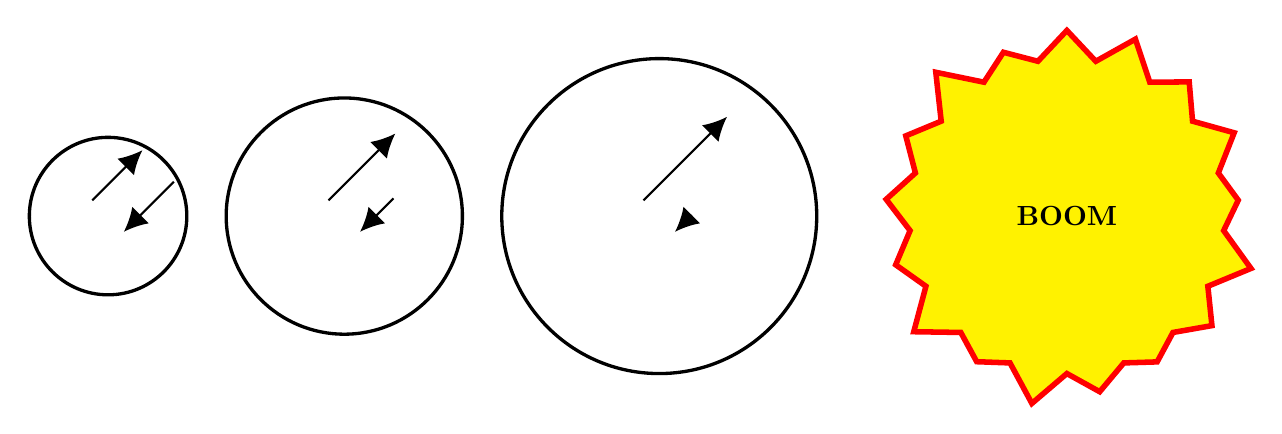
\begin{tikzpicture}
\drawstarforcebalance{0.0}{0.0}{1.0}{0.9}{0.9};
\drawstarforcebalance{3.0}{0.0}{1.5}{1.2}{0.6};
\drawstarforcebalance{7.0}{0.0}{2.0}{1.5}{0.3};
\node[starburst, fill=yellow, draw=red, line width=2pt, anchor=west, minimum size=5cm] at (10,0) {\textbf{BOOM}};
\end{tikzpicture}
\caption{\label{fig:nstars:star_explosion}%
A slight decrease $\dif \epsilon < 0$ in energy density weakens the gravitational force pulling a star in.
If the equation of state $\epsilon = \epsilon(P)$ in a star satisfies $\odv{P}/{\epsilon} < 0$, such a change in energy density would cause an increase $\dif P > 0$ in the pressure pushing the star out.
The greater pressure then causes the star to expand, which in turn causes another decrease in energy density.
Repeated application of the same argument shows that the star continues to expand while the pressure grows indefinitely, so the star ultimately explodes.
}
\end{figure}

From the expression $v = c \sqrt{\odv{P}/{\epsilon}}$ of the speed of sound, it also sounds reasonable to require that
\begin{equation}
	\odv{P}{\epsilon} > 0
\end{equation}
for it to be a real quantity.
Violation of this condition would in fact have dramatic consequences.
First, note that an increase in energy density $\dif \epsilon > 0$ always increase the gravitational force attempting to pull the star in.
If such an increase implied a \emph{decrease} $\dif P < 0$ in the pressure that pushes the star out, then the gravitational force would automatically ``win'', causing the star to contract, and hence the energy density to increase further.
Repeating the argument, we understand that the star collapses.
This process is illustrated in \cref{fig:nstars:stability_mass_pressure}.
Likewise, if a decrease $\dif \epsilon < 0$ caused an increase $\dif P > 0$, the same argument shows that the pressure wins and the star explodes.
However, if the two always change by the same sign, then the two forces will at the very least counteract each other instead of being driven apart.
In this case the star \emph{can} be stable, but the balance between the forces would have to be investigated in detail to conclude if it \emph{is}.
This criterion does not let us rule out any of our stars, either, but it will be useful to assume \TODO{ref} in the following.

\begin{figure}
\centering
\begin{tikzpicture}
\begin{axis}[axis x line=bottom, axis y line=left, xlabel=$P_0$, ylabel=$M$, xtick=\empty, ytick=\empty]
	\addplot[domain=-1:+1, black] {-x^2};

	\node [draw=black, circle, fill, inner sep=1pt, label=left:$E_1$] at (axis cs:-0.7,-0.49) {};
	\node [draw=black, circle, fill, inner sep=1pt, label=left:$E_2$] at (axis cs:-0.5,-0.25) {};
	\node [draw=black, circle, fill, inner sep=1pt, label=right:$C$ ] at (axis cs:-0.5,-0.49) {};

	\node [draw=black, circle, fill, inner sep=1pt, label=left:$E_2$] at (axis cs:+0.7,-0.49) {};
	\node [draw=black, circle, fill, inner sep=1pt, label=left:$E_1$] at (axis cs:+0.5,-0.25) {};
	\node [draw=black, circle, fill, inner sep=1pt, label=right:$C$ ] at (axis cs:+0.7,-0.25) {};
\end{axis}
\end{tikzpicture}
\caption{\label{fig:nstars:stability_mass_pressure}}
\end{figure}

A third necessary condition is
\begin{equation}
	\odv{M(P_0)}{P_0} > 0
\label{eq:nstars:stability_mass_pressure}
\end{equation}
for stars parametrized by their central pressure $P_0$.

Consider a star $E_1$ in equilibrium on the increasing part of the curve in \cref{fig:nstars:stability_mass_pressure}, where condition \eqref{eq:nstars:stability_mass_pressure} is satisfied.
Now compress this star to the non-equilibrium star $C$ with the same mass, and let $E_2$ be the star in equilibrium with the same central pressure as $C$.
Then $C$ has less mass than $E_2$, and hence weaker gravitational forces than $E_2$, but the same central pressure as $P_2$.
As a result, the star will expand and decrease its central density and pressure, causing it to return towards the equilibrium star $E_1$.

Let us we repeat the argument on the decreasing part of the curve, where condition \eqref{eq:nstars:stability_mass_pressure} does not hold.
After the compression from $E_1$ to $C$, we see that $C$ has more mass and hence stronger gravitational forces than $E_2$, but again the same central pressure.
The star therefore contracts, and repeating the argument causes it to collapse completely.

The criterion \eqref{eq:nstars:stability_mass_pressure} shows that the stars located between the maximum mass and the bottom of the spiral in \cref{fig:nstars:massradius} are unstable!

\subsection{General analysis}

The arguments presented above were necessary, but not sufficient for stellar stability.
Let us analyze the stability of the stars in a more rigorous way by finding a mathematical definition of stability.

In \cref{sec:einstein_to_tov}, we showed that in the spherically symmetric metric \eqref{eq:tov:metric} for a perfect fluid with energy-momentum \eqref{eq:tov:energy_momentum_perfect_fluid} in equilibrium with four-velocity $U^\mu = (U^0, \vec{0})$, the Einstein field equations \eqref{eq:einstein} reduced to
\begin{subequations}
\begin{align}
	\frac{1}{r^2} e^{-2 \beta_0} \left( 2 r \beta_0' - 1 + e^{2 \beta_0} \right)                         &= \frac{8 \pi G}{c^4} \epsilon_0        , \\
	\frac{1}{r^2} e^{-2 \beta_0} \left( 2 r \alpha_0' + 1 - e^{2 \beta_0} \right)                              &= \frac{8 \pi G}{c^4} P_0         , \\
	e^{-2 \beta_0} \left( \alpha_0'' + (\alpha_0')^2 - \alpha_0' \beta_0' + \frac{1}{r} (\alpha_0' - \beta_0') \right) &= \frac{8 \pi G}{c^4} P_0,
\end{align}
\label{eq:nstars:field_equations_equilibrium}
\end{subequations}
where we have used the subscript $0$ to indicate that these are all quantities in \emph{equilibrium}.
Suppose instead that the fluid is slightly perturbed from equilibrium with four-velocity $U^\mu = (U^0, U^1, 0, 0)$, now with non-zero radial component $U^1$.
Then the field equations change, and their solutions $\alpha(r,t)$, $\beta(r,t)$, $P(r,t)$ and $\epsilon(r,t)$ gains an additional time dependence.
Chandrasekhar found the new field equations, wrote the solutions
\begin{equation}
\begin{aligned}
	\alpha   (r, t) &= \alpha_0  (r) + \alpha_1  (r, t), & \qquad \qquad
	\beta    (r, t) &= \beta_0   (r) + \beta_1   (r, t), \\
	P        (r, t) &= P_0       (r) + P_1       (r, t), & \qquad \qquad
	\epsilon (r, t) &= \epsilon_0(r) + \epsilon_1(r, t). \\
\end{aligned}
\end{equation}
as small deviations $f_1(r,t)$ from their equilibria counterparts $f_0(r)$, expanded the field equations to first order in the deviations and subtracted the equilibrium equations \eqref{eq:nstars:field_equations_equilibrium} to simplify the system.
Defining $v = e^\alpha U^1$, he then obtained the system \TODO{ref chandrasekhar paper}
\begin{subequations}
\begin{align}
	(2 r e^{-2 \beta_0} \beta_1)' &= \frac{8 \pi G}{c^4} \epsilon_1 , \\
	r e^{-2 \beta_0} (2 \alpha_1' - 4 \alpha_0' \beta_1) &= 2 e^{-2 \beta_0} \beta_1 + \frac{8 \pi G}{c^4} r^2 P_1 , \\
	e^{-2 \beta_0} \dot{\beta_1} &= -\frac{8 \pi G}{c^4} (P_0 + \epsilon_0) r v ,
\end{align}
\end{subequations}
From the conservation $\nabla_\mu T^{\mu \nu} = 0$ from energy-momentum, he also obtained the complementary equation
\begin{equation}
	e^{2(\beta_0 - \alpha_0)} (P_0 + \epsilon_0) \dot{v} + P_1' + (P_0 + \epsilon_0) \alpha_1' + (P_1 + \epsilon_1) \alpha_0' = 0 .
\end{equation}
Finally, he defines $\dot{\xi} = v$ to distinguish the coordinate $r$ from the function $\xi(r, t)$ and assumes a solution on the form
\begin{equation}
	\xi(r,t) = \frac{e^\alpha}{r^2} U_n(r) e^{i \omega_n t} .
\end{equation}
Then $\xi(r,t)$ is a solution to the Einstein equations if $U_n(r)$ and the corresponding eigenvalue $\omega_n^2$ solves the \textbf{Sturm-Liouville problem}
\begin{equation}
	\odv*{ \left[ \Pi(r) \odv{U_n(r)}{r} \right] }{r} + \left[ Q(r) + \omega_n^2 W(r) \right] U_n(r) = 0 ,
\label{eq:nstars:sturm_liouville}
\end{equation}
where the coefficient functions are
\TODO{use big/small $u$/$U$ in ST-eq/4-vel}
\TODO{check units}
\begin{subequations}
\begin{align}
	\Pi &= \frac{1}{r^2} e^{\beta_0 + 3 \alpha_0} \gamma P_0 , \\
	Q   &= -\frac{4}{r^3} e^{\beta_0 + 3 \alpha_0} P_0' - \frac{8 \pi}{r^2} e^{3 \beta_0 + 3 \alpha_0} P (\epsilon_0 + P_0) + \frac{e^{\beta_0 + 3 \alpha_0}}{r^2(\epsilon_0 + P_0)} (P_0')^2 , \\
	W   &= \frac{1}{r^2} e^{3 \beta_0 + \alpha_0} (\epsilon_0 + P_0) .
\end{align}
\end{subequations}
The perturbation is assumed to take place adiabatically with the adiabatic index
\begin{equation}
	\gamma = \frac{\epsilon + P}{P} \odv{P}{\epsilon} ,
\end{equation}
and the boundary conditions are \TODO{cite ref catalogue}
\begin{equation}
	u(r) \propto r^3 \text{ at $r=0$}
	\qquad \text{and} \qquad
	u'(r) = 0 \text{ at $r=R$}.
\end{equation}
The boundary condition at $r=0$ is derived by observing that $r = 0$ is a regular singular point of the Sturm-Liouville equation \eqref{eq:nstars:sturm_liouville} so $U \propto r^3$ in order for $\xi$ and $\xi'$ to be finite there.
Physically, this implies that $\xi(0, t) = 0$, so the fluid at the center is not displaced, which is the only reasonable condition in a spherically symmetric situation.
At $r = R$, the boundary condition $u'(r) = 0$ follows from requiring that the Lagrangian variation in the pressure following a fluid element in the flow vanishes.

A characteristic feature of Sturm-Liouville problems is that the eigenvalues form a discrete, increasing sequence
\begin{equation}
	\omega_0^2 < \omega_1^2 < \omega_2^2 < \cdots .
\end{equation}
This enables us to make a rigorous definition of stellar stability.
\begin{itemize}
\item If $\omega_0^2 > 0$, then all vibration modes have $\omega_n^2 > 0$, so $\omega_n$ is real.
      Then $\xi_n(r, t) \propto e^{i \omega_n t}$ merely oscillates back and forth, so the star attempts to return to equilibrium, and we say the star is \textbf{stable}.
\item If $\omega_0^2 < 0$, then at least one vibration mode has $\omega_n = \pm i \abs{\omega_n}$, so $\omega_n$ is imaginary.
      Then $\xi(r,t) = \propto e^{\pm \abs{\omega_n} t}$ takes off exponentially, so the star either implodes or explodes, and we say the star is \textbf{unstable}.
\end{itemize}

\pgfplotstableread{../code/data/nmodes_norm.dat}{\nmodestable}
\pgfplotstablegetelem{0}{omega2}\of{\nmodestable}
got \pgfplotsretval

\pgfplotstablegetrowsof{\nmodestable}
\pgfmathparse{int(\pgfmathresult-1)}
\pgfplotstablegetelem{\pgfmathresult}{r}\of{\nmodestable}
\pgfmathsetmacro{\maxR}{\pgfplotsretval}
radius is \maxR

\usetikzlibrary{calc}
\begin{figure}
\begin{tikzpicture}
\begin{groupplot}[
	group style={group size=2 by 1, horizontal sep=5pt},
	width=8cm, height=7cm,
	xlabel=$r / R$,
	xmin=-0.1, xmax=1.1, ymin=-1.1, ymax=+1.1, restrict y to domain=-100:+100,
	xtick={0,0.5,1}, ytick={-1,0,1},
	ymajorgrids=true,
	no markers, cycle list name=color list, % or exotic
]
\nextgroupplot[
	ylabel=$U_n / \norm{U_n}_\infty$,
	legend cell align=left, legend columns=5, legend style={at={(1.0, 1.03)}, anchor=south},
]
\pgfplotstableread{../code/data/nmodes_norm.dat}{\nmodestable};
\pgfplotsinvokeforeach{0,1,2,3,4} {
	\addplot+ [thick] table [x expr=\thisrow{r}/\maxR, y=U#1] {\nmodestable};
	\pgfplotstablegetelem{#1}{omega2}\of{\nmodestable}
	\addlegendentryexpanded{$\omega_{#1}^2 = \pgfmathprintnumber[fixed, fixed zerofill, precision=2]{\pgfplotsretval}$};
}

\nextgroupplot[
	ylabel=$U_n / \norm{U_0}_\infty$, yticklabel pos=right, ylabel near ticks,
	yticklabels={},
];
\tablemaximum{../code/data/nmodes.dat}{U0}{\maxU}{r}{\maxr}
\pgfplotsinvokeforeach{0,1,2,3,4} {
	\addplot+ [thick] table [x expr=\thisrow{r}/\maxR, y expr=\thisrow{U#1}/\maxU] {../code/data/nmodes.dat};
}
\addplot [dashed, domain=0:0.5, restrict y to domain=0:1.1, samples=50] {(x*\maxR)^3 / \maxU} node[pos=0.6, label={[xshift=+1ex]135:$\propto r^3$}] {};
\end{groupplot}
\end{tikzpicture}
\end{figure}

\begin{figure}
\begin{tikzpicture}
\pgfplotstableread{../code/data/shoot.dat}{\shoottable}
\pgfplotstablegetrowsof{\shoottable}
\pgfmathparse{int(\pgfplotsretval-1)}
\pgfplotstablegetelem{\pgfmathresult}{r}\of{\shoottable}
\pgfmathsetmacro{\maxR}{\pgfplotsretval}
\begin{axis}[
	width=11cm, height=8cm,
	xlabel=$r/R$, ylabel=$U(r) / \norm{U_0(r)}_\infty$,
	title={Convergence of $U(r; \omega^2) \rightarrow U_0(r; \omega_0^2)$ \\ with the shooting method},
	%every axis title/.style={at={(0.5,1)}, align=center, above=1ex, text width=0.8*\pgfkeysvalueof{/pgfplots/width}]},
	ymin=-2.1, ymax=+2.1,
	xtick distance=0.25, ytick distance=1,
	ymajorgrids, xmajorgrids,
	cycle list name=color list,
	legend style={anchor=south west, at={(1.02, 0)}},
	legend cell align=right,
	colormap name=blackred, cycle list={[samples of colormap=33]},
]
\addlegendimage{empty legend}
\addlegendentry{\hspace{-0.6cm}\textbf{Value of $\omega^2$}} % hack for legend title: https://tex.stackexchange.com/questions/2311/add-a-legend-title-to-the-legend-box-with-pgfplots
\pgfplotsinvokeforeach{0,...,32}{ % 32, it works but it is very slow
	\pgfplotstablegetelem{#1}{omega2}\of{../code/data/shoot.dat}
	\addplot+ [thick, restrict y to domain=-5:5] table [x expr=\thisrow{r}/\maxR, y expr={\thisrow{U#1} / 0.000312}] {../code/data/shoot.dat}; % faster to read directly from file for some reason
	\addlegendentryexpanded{$\pgfmathprintnumber[precision=10, fixed, fixed zerofill]{\pgfplotsretval}$};
}
\end{axis}
\end{tikzpicture}
\caption{\label{fig:nstars:shooting_convergence}%
	The shooting method is used to determine the squared frequency $\omega_N^2$ of the vibration mode $U_N(r)$ with $N=0$ of a neutron star with central pressure $P_0 = 10^3 \epsilon_0$.
	First, it finds two values $\omega_-^2 = -16$ and $\omega_+^2 = 0$ whose corresponding solutions $U(r)$ have $n_- \leq N$ and $n_+ > N$ nodes, respectively.
	The exact squared frequency is then guaranteed to lie in $\omega_-^2 < \omega^2 < \omega_+^2$.
	Next, the algorithm finds the solution $U(r)$ corresponding to $\omega^2 = (\omega_-^2 + \omega_+^2) / 2 = -8$ and counts its number of nodes.
	Here, it is found to have $n > N$ nodes, so $\omega_+^2 = -8$ gives a tighter upper bound on $\omega^2$ than $0$.
	In the opposite case $n \leq N$, it would have been a better lower bound $\omega_-^2 = -8$.
	Moving on, the algorithm continues to split intervals in this fashion until the lower and upper bounds are so close that any value in the interval $[\omega_-^2, \omega_+^2]$ is satisfactory.
}
\end{figure}

\subsection{Sufficient conditions for stability}

\TODO{discuss mass bound}

\TODO{compare with earlier results, most massive neutron stars}

\TODO{stability analysis, which parts of the plot are meaningful?}

\TODO{keywords: $dp/d\epsilon = 1/3$ = conformal limit? no mass in this EOS = scale invariance. $T^{\mu \nu}$ traceless?}
